\begin{pastexam}[label={px:gk3-108-ds-02}]{高考三級資訊處理 108 年 第二題}
（申論；25 分）

給予如下二元樹節點的宣告，寫一 C 的遞迴程式 \texttt{swapTree（NODEPTR tree）}將每一節點的左、右節點互換
（Swap the left and right children of every node of a binary tree）。（25 分）
\begin{minted}[fontsize=\small,frame=single]{c}
struct node{
   int info;
   struct node *left;
   struct node *right;
}
typedef struct node *NODEPTR;

void swapTree(NODEPTR tree){

}
\end{minted}
\end{pastexam}

\begin{pastsoln}
（題目的 \texttt{struct node\{...\}} 右大括號後面少了分號，下面的程式補上。）

\textbf{想法。} 把整棵樹左右互換（鏡像），就是先把根的左右兩個指標對調，再對兩棵子樹各自做同一件事。
空樹什麼都不用做，是遞迴的終止條件。
\begin{minted}[fontsize=\small]{c}
struct node {
    int info;
    struct node *left;
    struct node *right;
};
typedef struct node *NODEPTR;

void swapTree(NODEPTR tree)
{
    NODEPTR temp;

    if (tree == NULL)                 /* 空樹：不用換 */
        return;
    temp = tree->left;                /* 對調根的左右子樹 */
    tree->left = tree->right;
    tree->right = temp;
    swapTree(tree->left);             /* 兩棵子樹各自互換 */
    swapTree(tree->right);
}
\end{minted}
先換再遞迴或先遞迴再換都可以（前序或後序的順序），結果相同；只要每個節點的兩個指標恰好對調一次。
不能用中序（先遞迴左、再換、再遞迴右），因為換完之後原本的左子樹跑到右邊，會被換兩次、原本的右子樹
一次都沒換。

\textbf{正確性}（對節點數歸納）。 空樹的鏡像是自己，正確。 非空樹 $T$ 的鏡像是：根不變，左子樹是 $T_R$
的鏡像、右子樹是 $T_L$ 的鏡像。 程式先讓 \texttt{left} 指向 $T_R$、\texttt{right} 指向 $T_L$，再由歸納假設
把兩棵子樹各自變成鏡像，正好符合定義。

\textbf{例子。}
\begin{center}
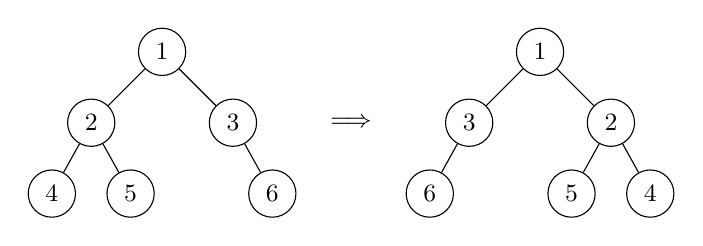
\begin{tikzpicture}[every node/.style={circle,draw,minimum size=6mm,inner sep=0pt,font=\small},
  level distance=9mm, level 1/.style={sibling distance=18mm}, level 2/.style={sibling distance=10mm}]
\node at (0,0) {1}
  child {node {2} child {node {4}} child {node {5}}}
  child {node {3} child[missing] child {node {6}}};
\node[draw=none] at (2.4,-0.9) {$\Longrightarrow$};
\node at (4.8,0) {1}
  child {node {3} child {node {6}} child[missing]}
  child {node {2} child {node {5}} child {node {4}}};
\end{tikzpicture}
\end{center}
左圖中序是 $4, 2, 5, 1, 3, 6$，互換後中序是 $6, 3, 1, 5, 2, 4$，恰好反過來——鏡像的中序就是原中序倒過來。

\textbf{複雜度。} 每個節點和每個空指標各呼叫一次，每次常數時間，時間 $O(n)$；遞迴深度是樹高，空間
$O(h)$。
\end{pastsoln}
